% chapters/chapter3/3_4_nmpc_results.tex
% !TeX root=../../main.tex

% NMPC Results and Architecture Evaluation
\section{ارزیابی کنترل‌کنندهٔ پیش‌بین مدل غیرخطی (\lr{NMPC})}

با توجه به محدودیت‌های اثبات‌شده برای کنترل کلاسیک، در این بخش عملکرد کنترل‌کنندهٔ پیش‌بین مدل غیرخطی ارزیابی می‌شود. این استراتژی بر پایهٔ حل برخط یک مسئلهٔ بهینه‌سازی مقید استوار است و از مکانیزم تغییر طول کابل به عنوان یک عملگر فعال (\lr{Active Damping}) بهره می‌برد.

% Basic NMPC Step Response
\subsection{تحلیل نتایج فاز پایه: ردیابی ورودی پله}

به منظور اعتبارسنجی اولیهٔ کنترل‌کننده، سیستم در یک حلقهٔ فیدبک گسسته (شکل \ref{fig:nmpc_basic_block}) تحت یک ورودی پله برای جابجایی انتقال $0.5$ متری و از شرایط سکون مورد آزمایش قرار گرفت.

\begin{figure}[hbt!]
    \centering
    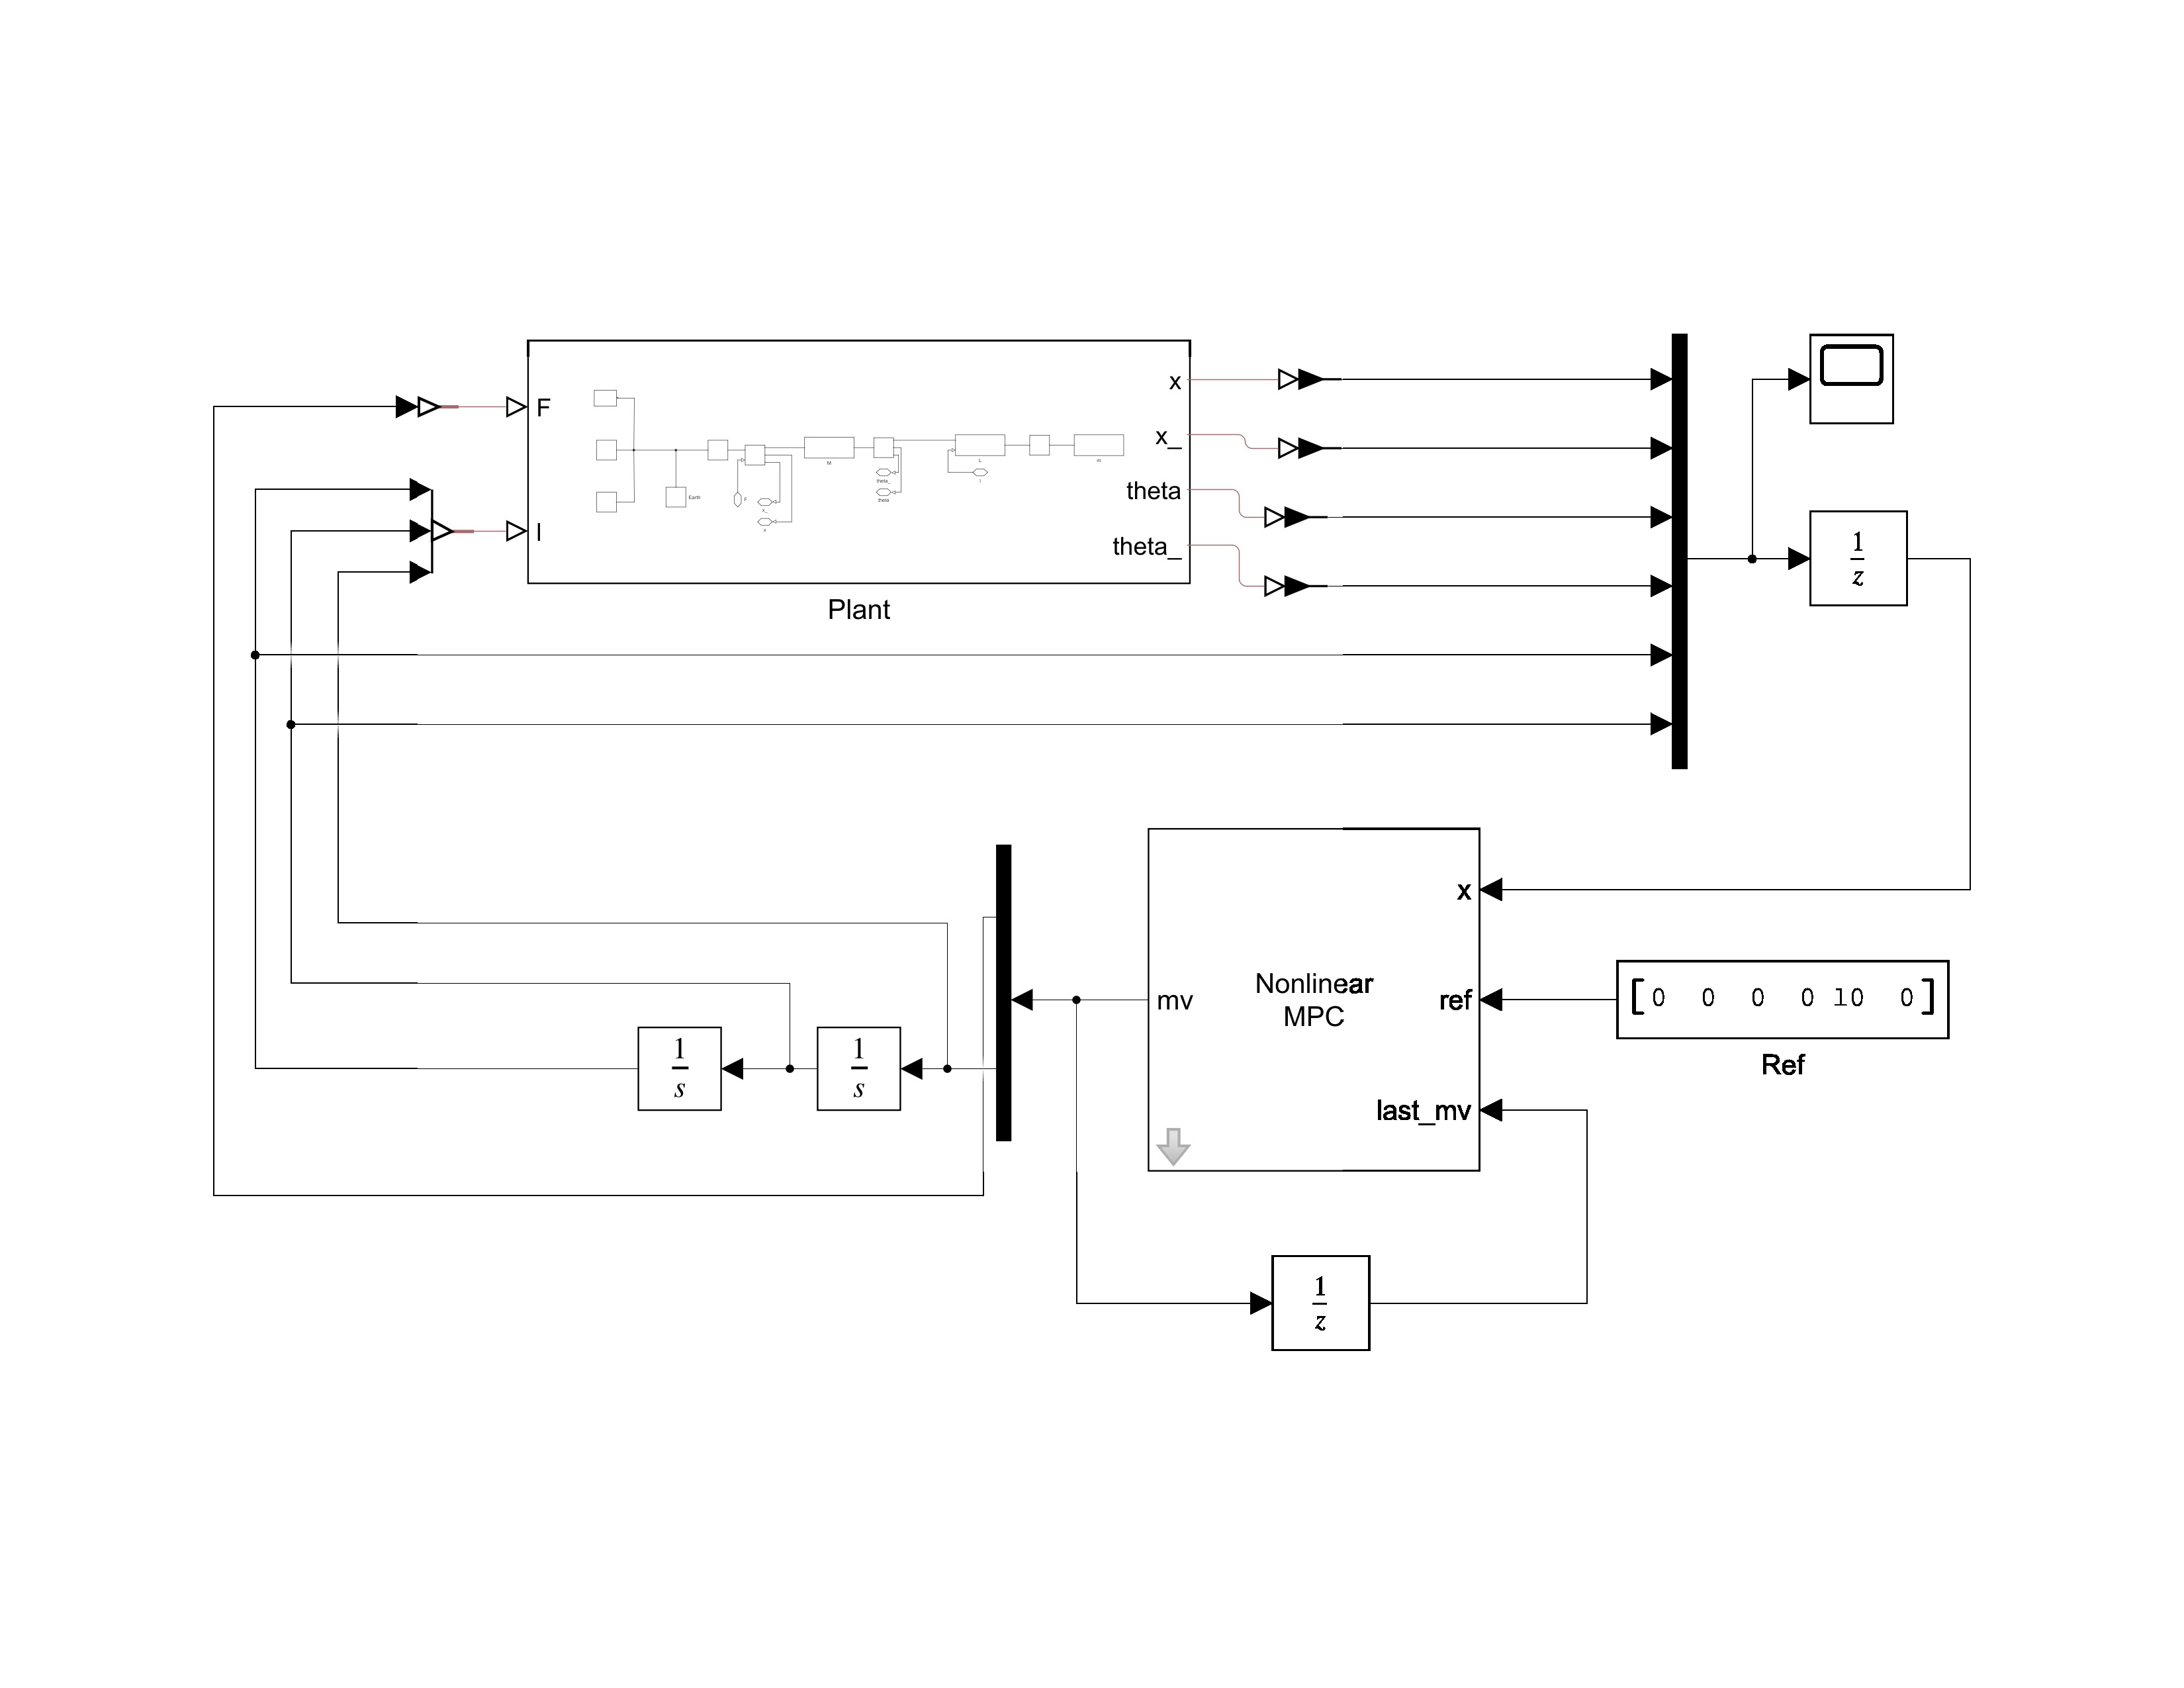
\includegraphics[width=0.9\textwidth]{images/3_NMPC_Basic/MPC_block_diagram.png}
    \caption{معماری حلقهٔ فیدبک کنترل‌کنندهٔ پیش‌بین غیرخطی پایه در ارتباط با مدل فیزیکی}
    \label{fig:nmpc_basic_block}
\end{figure}

نتایج شبیه‌سازی در شکل (\ref{fig:nmpc_basic_results}) نشان می‌دهد که کنترل‌کنندهٔ \lr{NMPC} به دلیل داشتن وزن غالب بر خطای موقعیت، کالسکه را با شیبی ملایم و کنترل‌شده به سمت نقطهٔ هدف هدایت می‌کند. نکتهٔ قابل توجه، رفتار متغیرهای زاویهٔ نوسان (\lr{$\theta$}) و طول کابل (\lr{$l$}) است. سیستم با استفادهٔ هوشمندانه از مکانیزم تغییر طول کابل، انرژی نوسانی پاندول را پیش از رسیدن به مرزهای ناپایداری جذب کرده و دامنهٔ نوسانات را در محدوده‌ای بسیار کوچک (به مراتب کمتر از قید ۱۵ درجه) محصور نگه می‌دارد. همگرایی سریع زاویهٔ نوسان به صفر هم‌زمان با توقف کالسکه، کارایی بالای الگوریتم بهینه‌سازی غیرخطی را به اثبات می‌رساند.

\begin{figure}[hbt!]
    \centering
    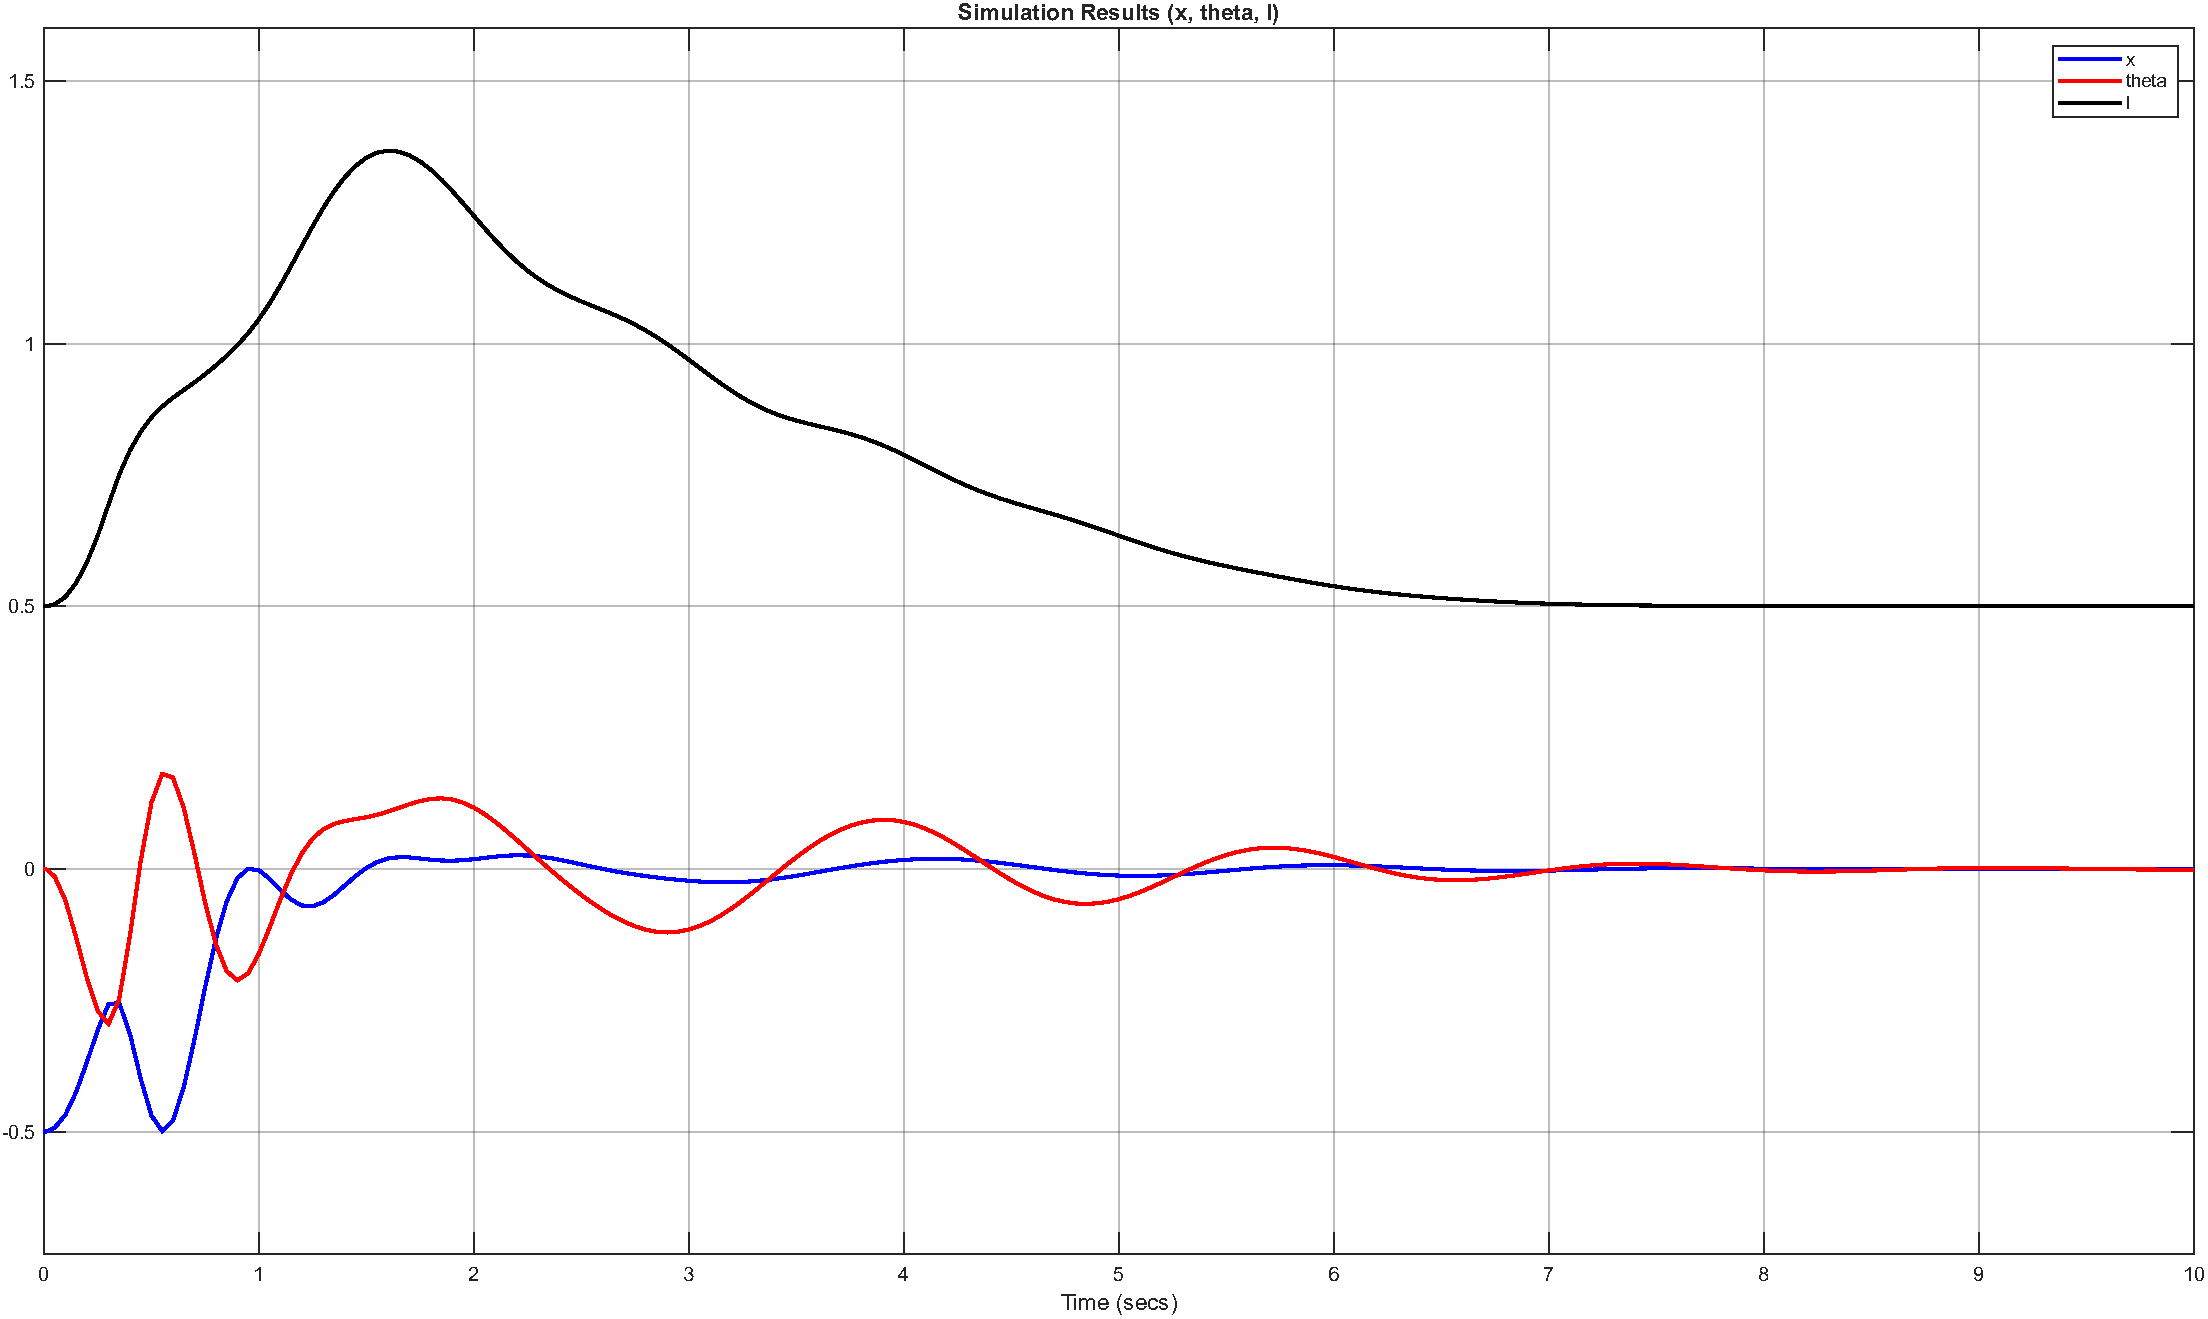
\includegraphics[width=0.8\textwidth]{images/3_NMPC_Basic/Simulation_Results_x_theta_l.pdf}
    \caption{پاسخ زمانی موقعیت کالسکه، زاویهٔ نوسان و طول کابل تحت ورودی پله}
    \label{fig:nmpc_basic_results}
\end{figure}

سیگنال‌های کنترلی تولیدشده (ورودی‌های پلنت) در شکل (\ref{fig:nmpc_basic_inputs}) رسم شده‌اند. مقادیر هر دو سیگنال به خوبی در بازهٔ نوسانی بین ۳- تا ۳ قرار گرفته‌اند که نشان می‌دهد عملگرها با حاشیهٔ امنیت بالایی درون محدوده‌های سخت‌افزاری تعریف‌شده ($50\mathrm{\ N}$ و $5\mathrm{\ m/s^2}$) عمل کرده و دچار اشباع (\lr{Saturation}) نشده‌اند.

\begin{figure}[hbt!]
    \centering
    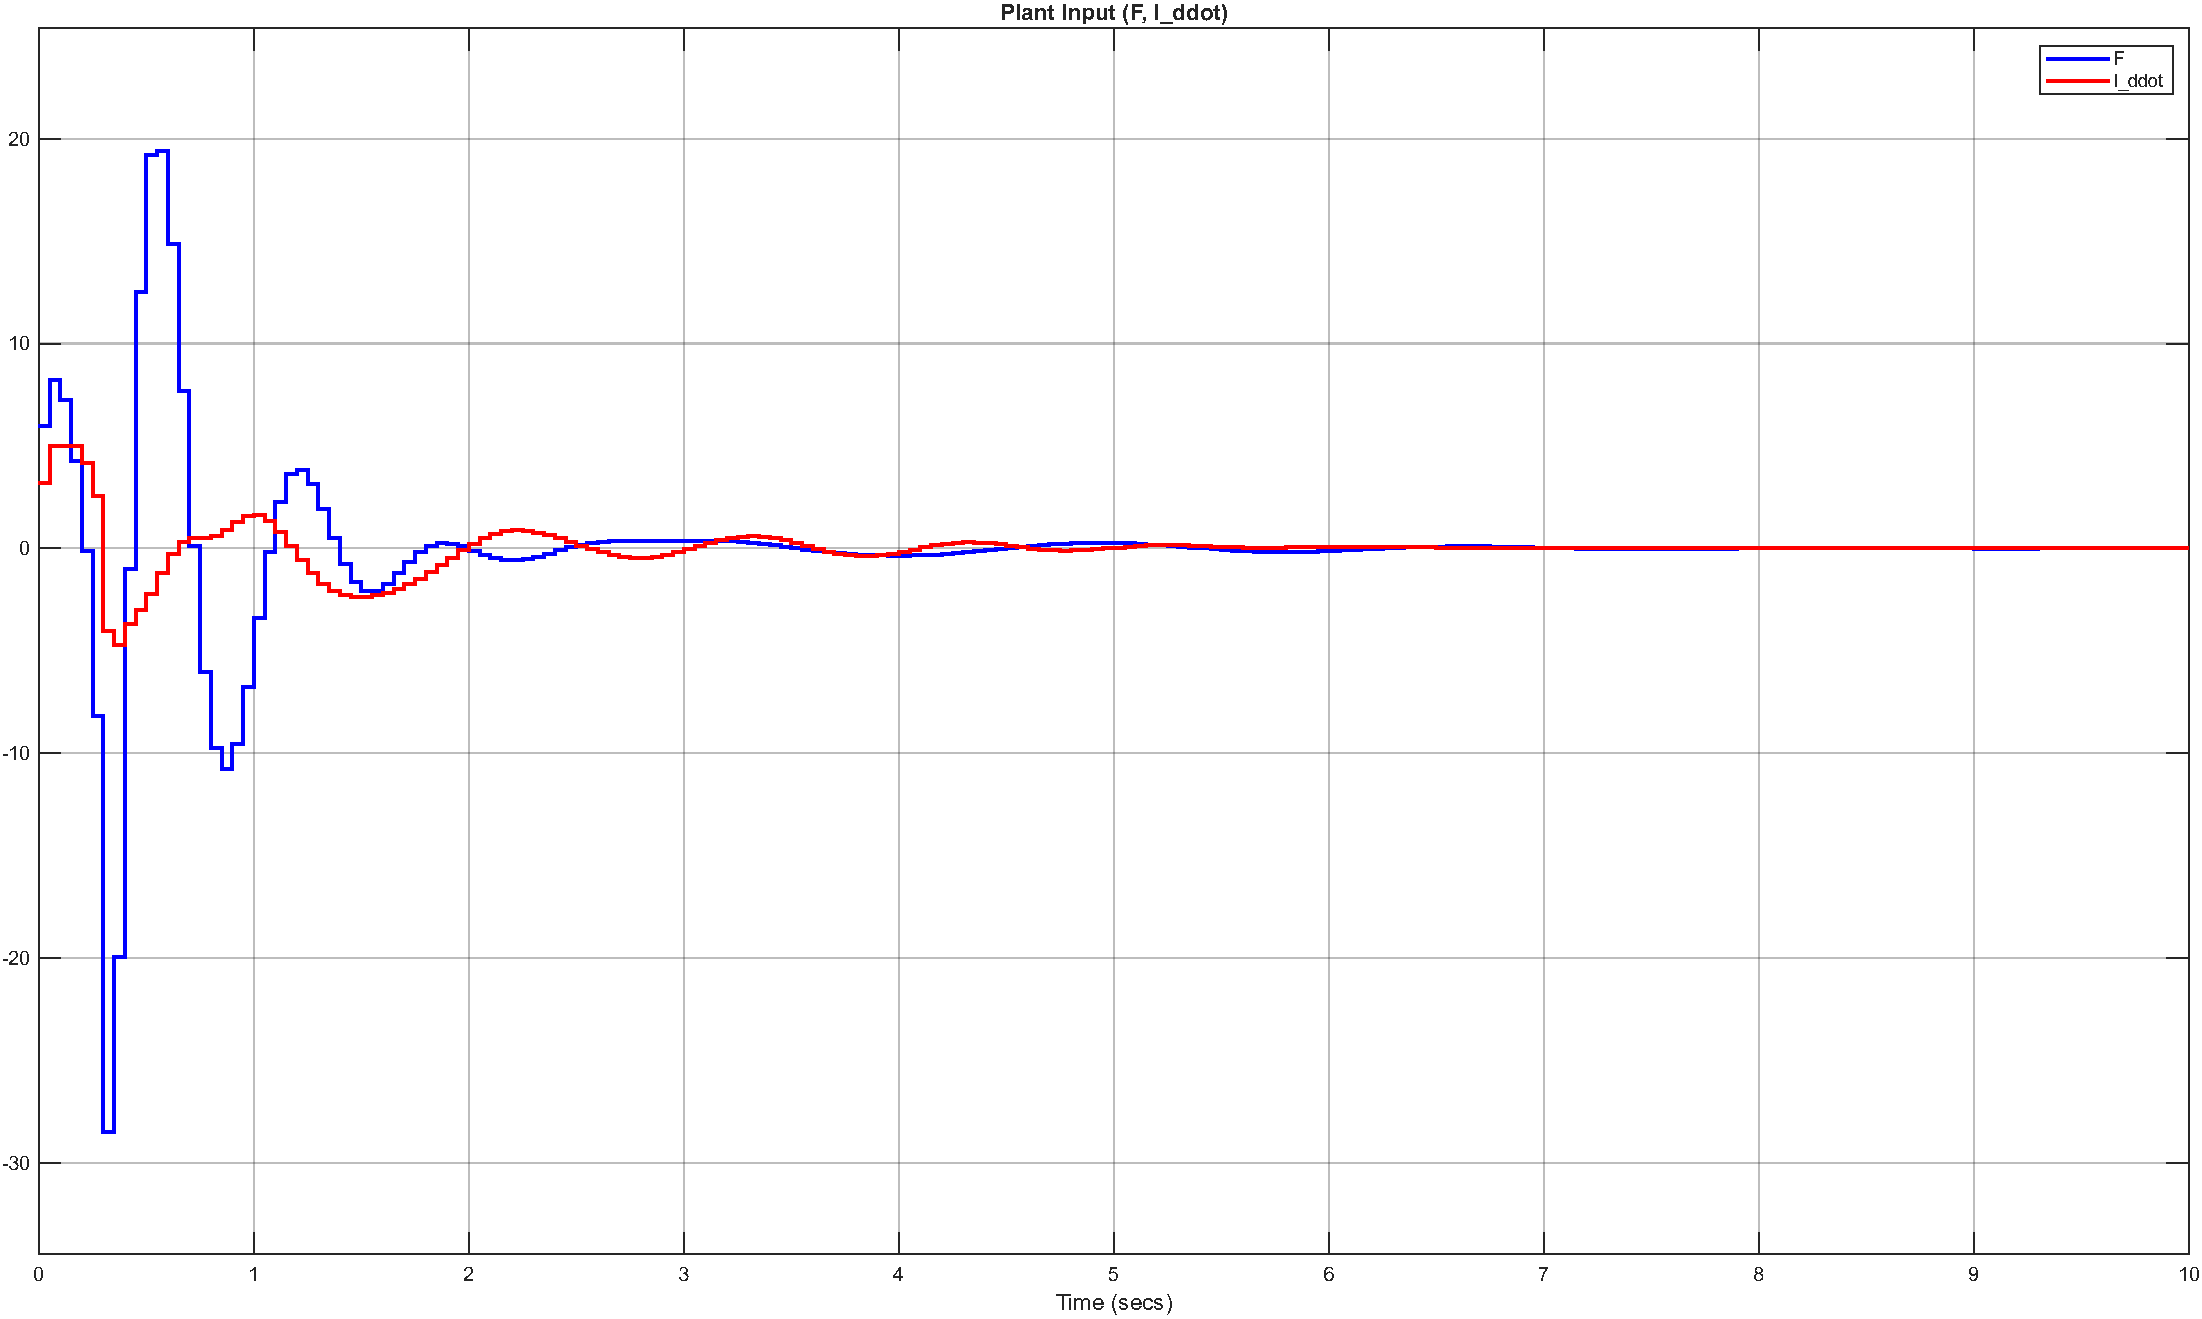
\includegraphics[width=0.8\textwidth]{images/3_NMPC_Basic/plant_input_F_l_ddot.pdf}
    \caption{سیگنال‌های کنترلی پایه: نیروی کالسکه (\lr{$F$}) و شتاب تغییر طول کابل (\lr{$\ddot{l}$})}
    \label{fig:nmpc_basic_inputs}
\end{figure}

% Need for Trajectory and Interference Paradox
\subsection{ضرورت استفاده از برنامه‌ریز مسیر و چالش تداخل فیدفوروارد}

اعمال یکبارهٔ خطای بزرگ موقعیت ($e = x_{ref} - x_0$) به شکل پله برای جابجایی‌های طولانی‌تر (نظیر ۵ متر)، کنترل‌کننده را وادار به درخواست حداکثر نیروی ممکن در لحظهٔ آغازین می‌کند. این امر به اشباع سریع عملگرها و تولید سیگنال‌های نوسانی و در نهایت ناپایداری سیستم می‌انجامد. برای حل این مشکل، مرجع پله به یک پروفایل حرکتی کاملاً نرم (\lr{S-Curve}) تبدیل شد (شکل \ref{fig:nmpc_traj_ref}).

\begin{figure}[hbt!]
    \centering
    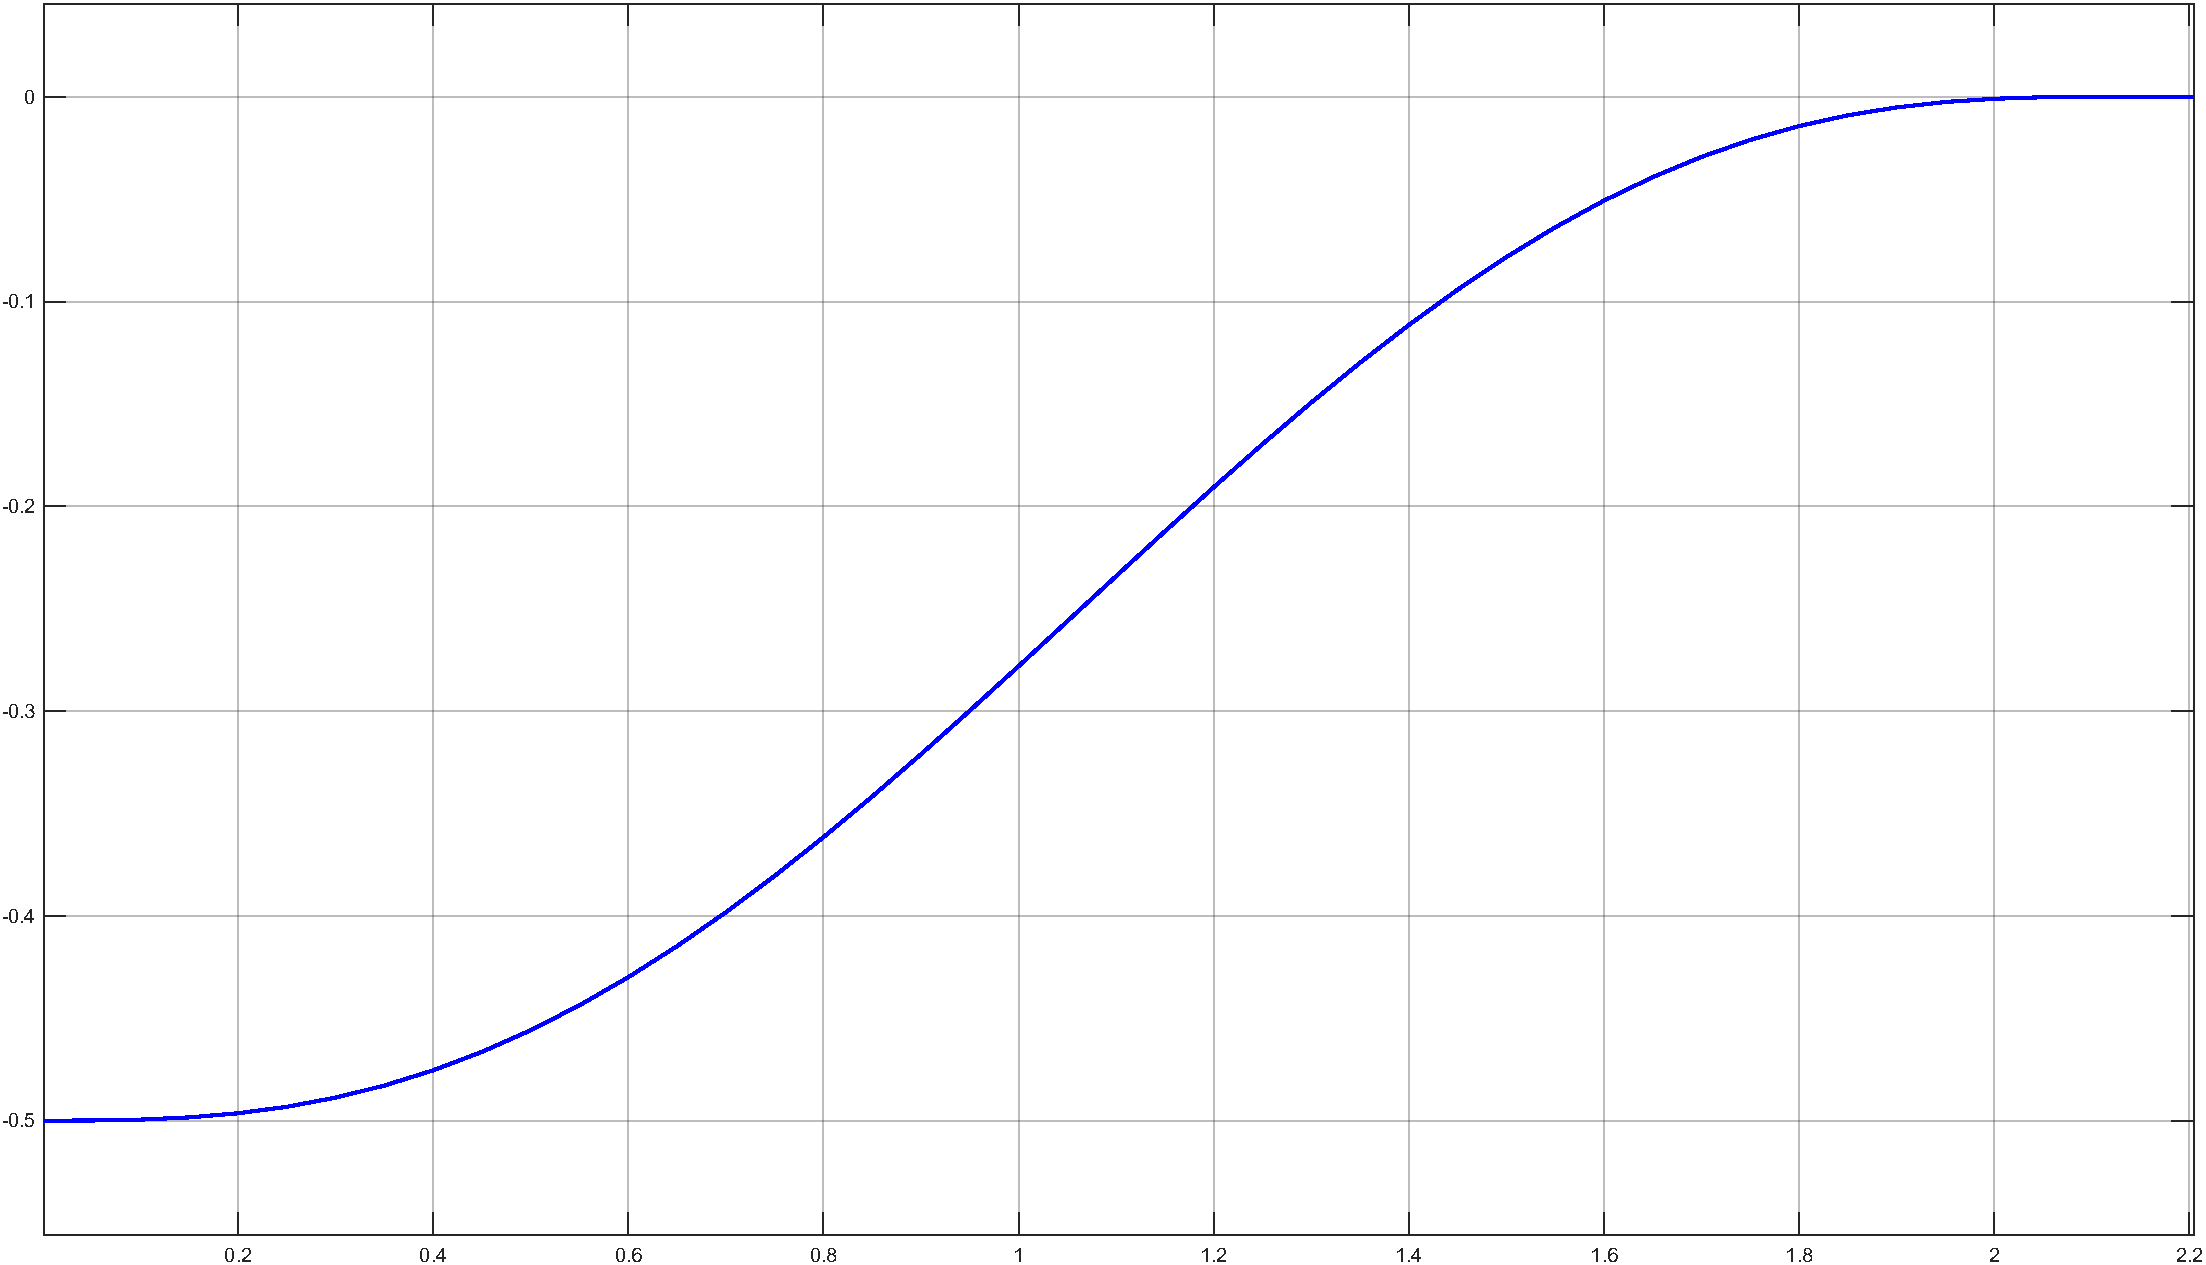
\includegraphics[width=0.75\textwidth]{images/4_NMPC_Trajectory/MPC_TRAJ_REF.pdf}
    \caption{پروفایل مسیر مرجع نرم تولیدشده توسط برنامه‌ریز سینماتیکی}
    \label{fig:nmpc_traj_ref}
\end{figure}

در فاز توسعهٔ این معماری، تلاش شد تا فیدفوروارد تحلیلی در کنار \lr{NMPC} پیاده‌سازی شود. اما این رویکرد به دلیل یک پارادوکس بنیادین با شکست مواجه شد: هدف اصلی \lr{NMPC} حفظ زاویهٔ نوسان در مقدار صفر است. با اعمال نیروی فیدفوروارد، سیستم شروع به شتاب‌گیری می‌کند و \lr{NMPC} با پیش‌بینی انحراف قطعی آونگ، از طریق اعمال یک نیروی منفی شدید با فیدفوروارد مقابله کرده و مانع حرکت کالسکه می‌شود.

برای رفع این تداخل، فیدفوروارد خارجی حذف شد و مسیر نرم آینده مستقیماً به عنوان مرجع به بهینه‌ساز تزریق گردید (شکل \ref{fig:nmpc_traj_block}). با افزایش افق پیش‌بینی، سالور \lr{NMPC} خود نقش فیدفوروارد را ایفا کرده و سیگنال‌های پیش‌دستانه‌ای (\lr{Proactive}) برای حرکت کالسکه و میراسازی نوسانات تولید می‌کند.

\begin{figure}[hbt!]
    \centering
    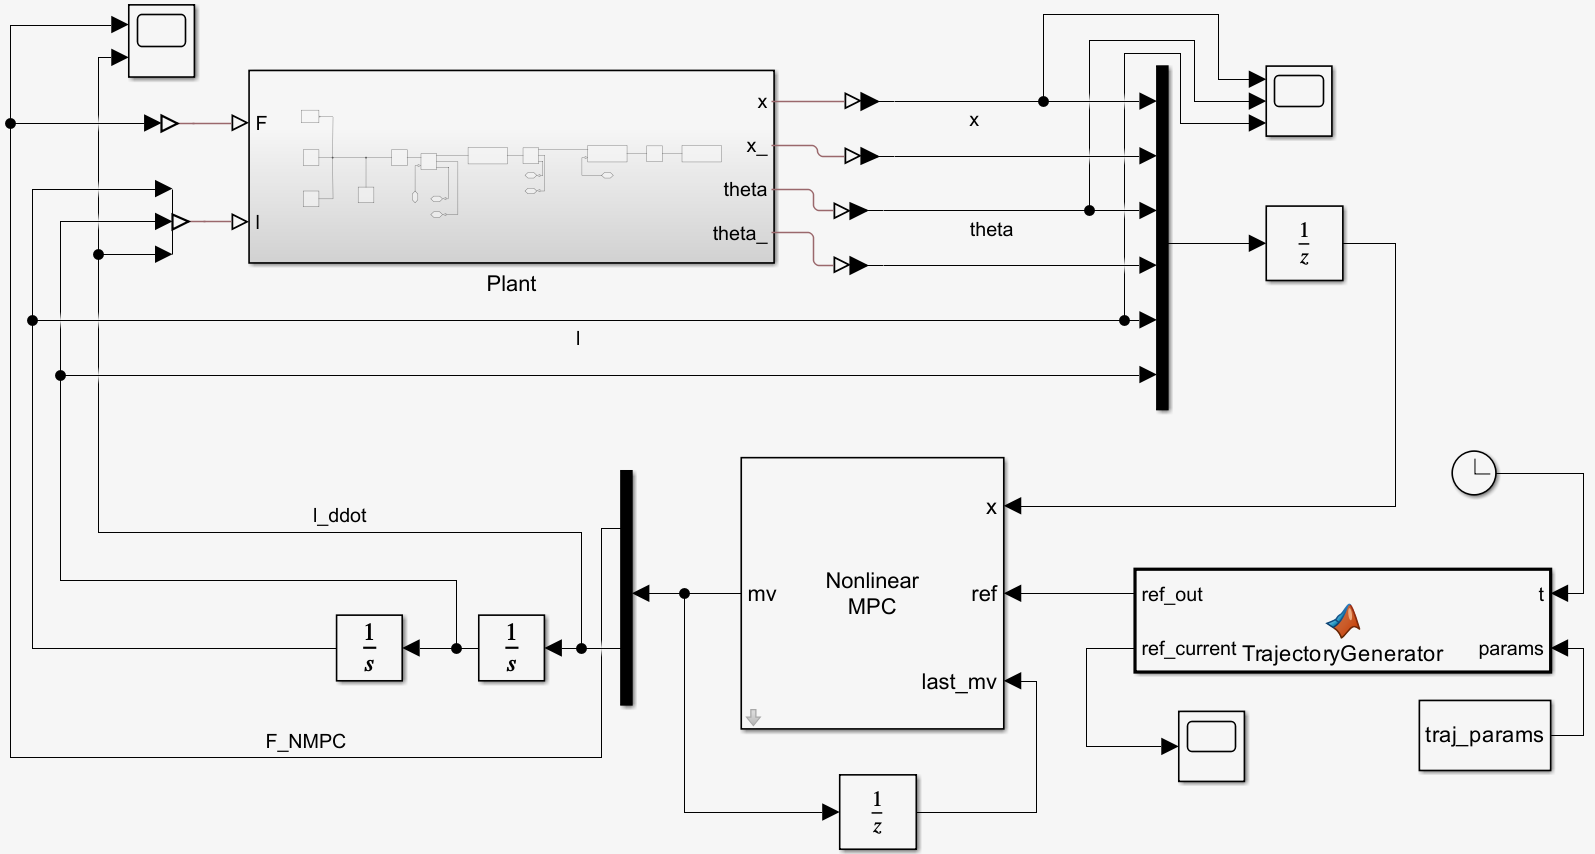
\includegraphics[width=0.95\textwidth]{images/4_NMPC_Trajectory/MPC_TRAJ_block_diagram.png}
    \caption{معماری نهایی حلقهٔ کنترل پیش‌بین یکپارچه فاقد فیدفوروارد خارجی}
    \label{fig:nmpc_traj_block}
\end{figure}

% Final Architecture Results
\subsection{تحلیل نتایج شبیه‌سازی با معماری ردیاب مسیر یکپارچه}

برای اثبات کارایی این معماری یکپارچه، سیستم تحت دو سناریوی جابجایی کوتاه و بلند ارزیابی شد.

\subsubsection{سناریوی جابجایی کوتاه‌برد ($0.5$ متر)}

در شکل (\ref{fig:nmpc_traj_05_states})، موقعیت کالسکه با دقت بالا و بدون فراجهش به هدف رسیده است. مهم‌ترین دستاورد این ساختار، سرکوب مطلق نوسانات پسماند است؛ \lr{NMPC} با استفاده از تغییرات نرم طول کابل، نوسانات را در طول حرکت میرا کرده و در لحظهٔ توقف کالسکه، آونگ نیز در وضعیت سکون کامل قرار دارد. سیگنال‌های کنترلی (شکل \ref{fig:nmpc_traj_05_inputs}) نیز رفتاری کاملاً نرم و به دور از مرزهای اشباع (در محدودهٔ $1.5$ تا $-1.5$) نشان می‌دهند.

\begin{figure}[hbt!]
    \centering
    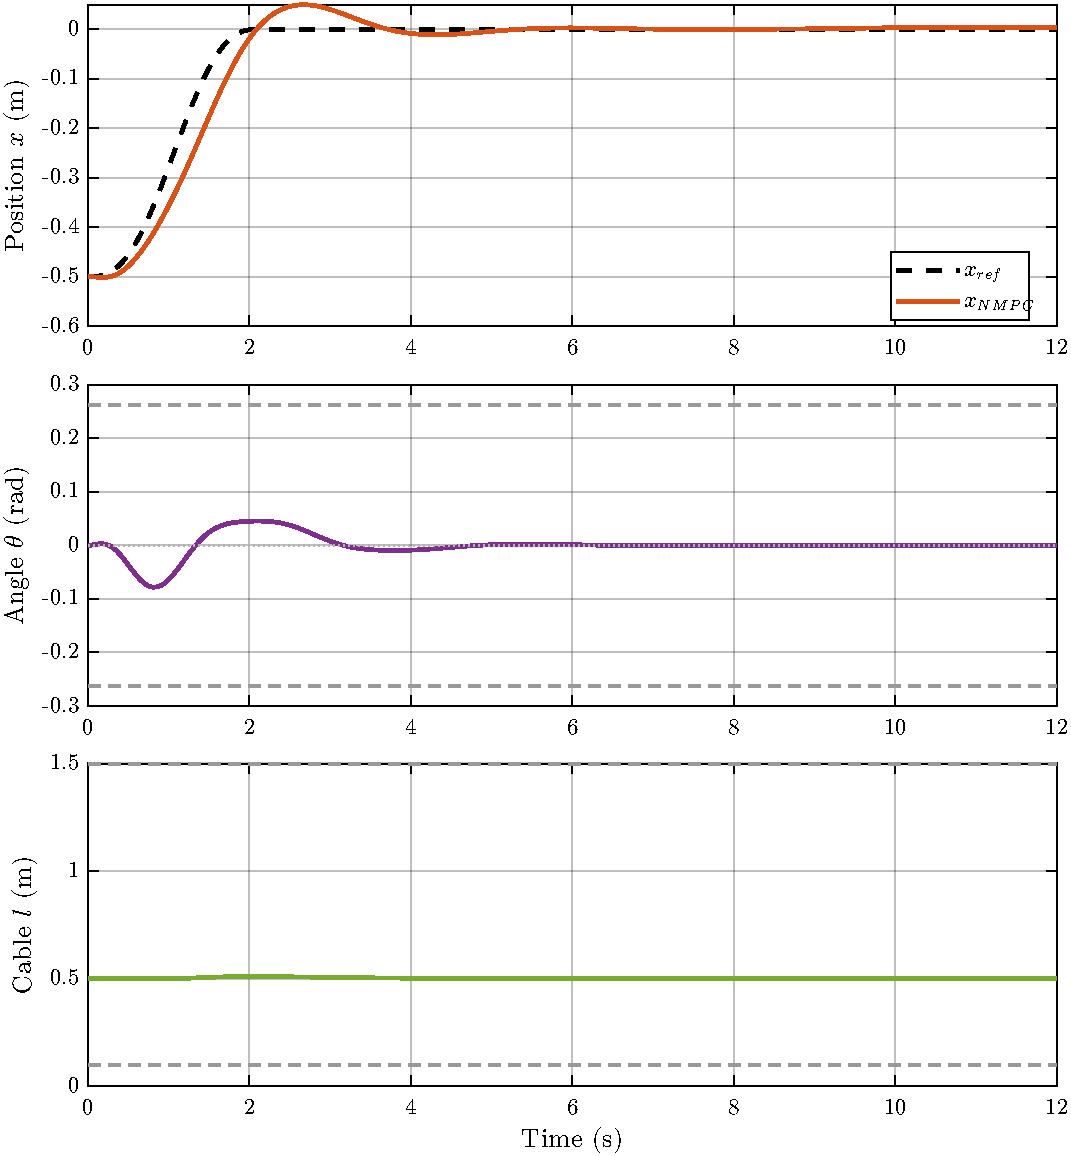
\includegraphics[width=0.85\textwidth]{images/4_NMPC_Trajectory/MPC_TRAJ_x_theta_l.pdf}
    \caption{پاسخ زمانی موقعیت، زاویه و طول کابل در معماری یکپارچه (جابجایی $0.5$ متر)}
    \label{fig:nmpc_traj_05_states}
\end{figure}

\begin{figure}[hbt!]
    \centering
    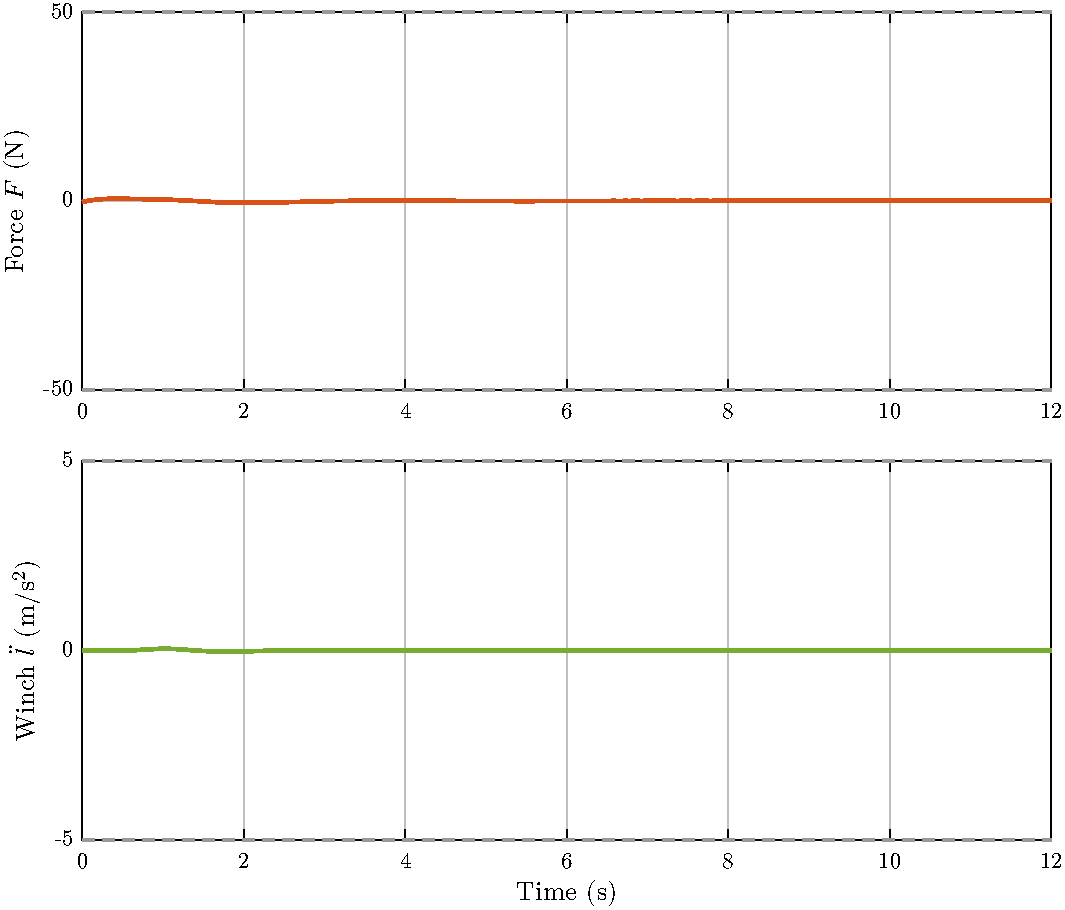
\includegraphics[width=0.85\textwidth]{images/4_NMPC_Trajectory/MPC_TRAJ_f_l_ddot.pdf}
    \caption{سیگنال‌های کنترلی بهینه‌سازی‌شده برای جابجایی $0.5$ متر}
    \label{fig:nmpc_traj_05_inputs}
\end{figure}

\subsubsection{سناریوی جابجایی بلندبرد ($5$ متر) و آزمون مقیاس‌پذیری}

در چالش‌برانگیزترین ارزیابی (جابجایی ۵ متری)، سیستم بر خلاف حالت پایه پایدار باقی می‌ماند (شکل \ref{fig:nmpc_traj_5_states}). زاویهٔ آونگ در طول این مسیر، با وجود شتاب‌گیری‌های ممتد، در بازهٔ بسیار امنی کنترل شده و در زمان توقف، سیستم بدون هیچ‌گونه نوسان پسماندی در آرامش کامل قرار می‌گیرد.

پروفایل سیگنال‌های کنترلی (شکل \ref{fig:nmpc_traj_5_inputs}) حاکی از آن است که الگوریتم برای غلبه بر اینرسی مسیر طولانی، نیروی بیشتری اعمال کرده است، اما همچنان با فاصلهٔ ایمنی از مرز محدودیت فیزیکی قرار دارد. ترکیب هوشمندانهٔ نیروی کالسکه و متغیر شتاب کابل توسط سالور واحد، پایداری و ایمنی مطلق سیستم را در سخت‌ترین شرایط حرکتی تضمین می‌کند.

\begin{figure}[hbt!]
    \centering
    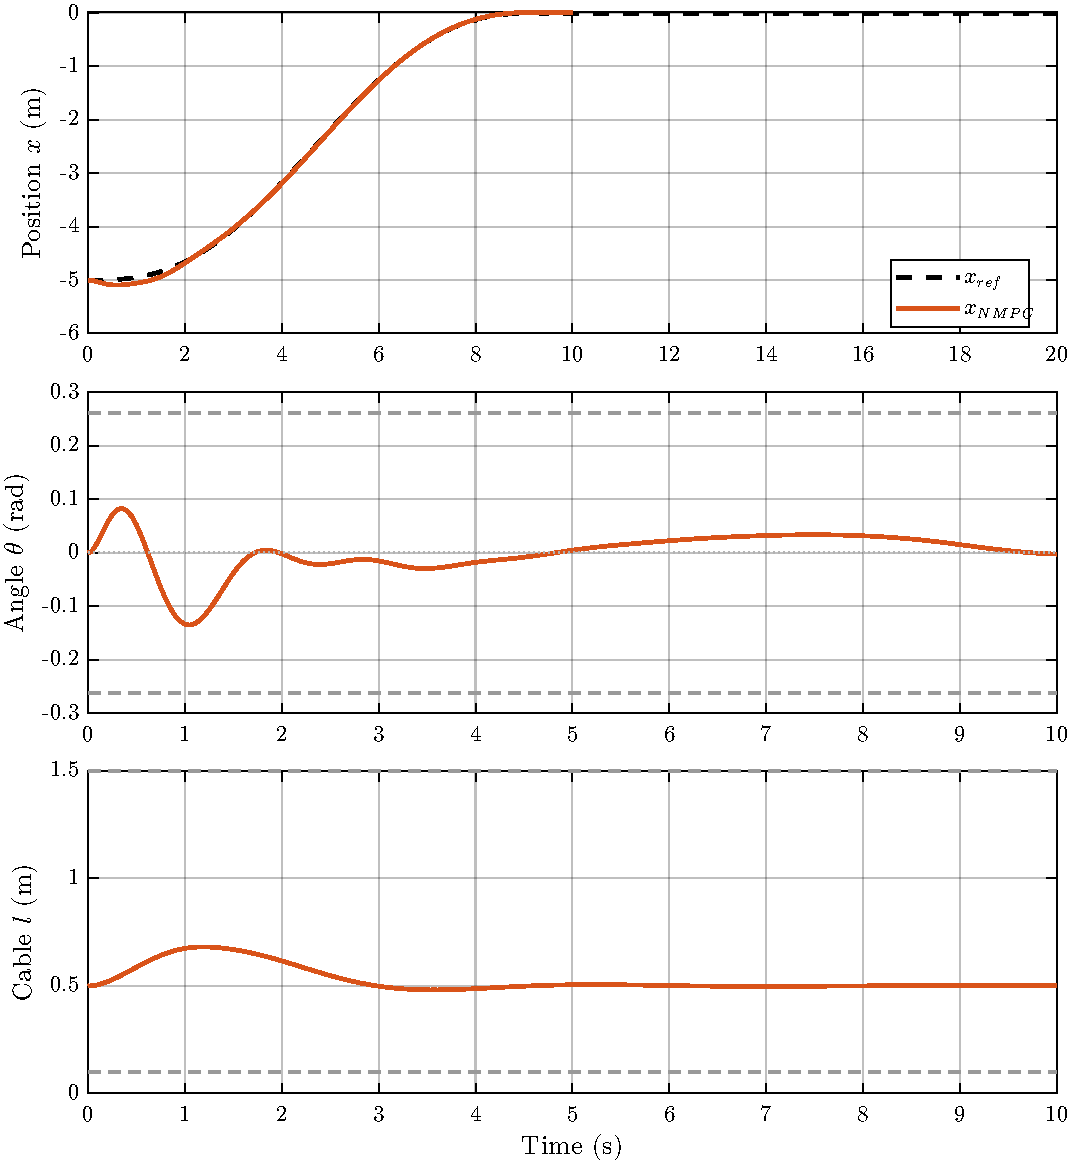
\includegraphics[width=0.85\textwidth]{images/4_NMPC_Trajectory/MPC_TRAJ_x_theta_l_5.pdf}
    \caption{ردیابی دقیق و حذف کامل نوسانات پسماند در جابجایی ۵ متر}
    \label{fig:nmpc_traj_5_states}
\end{figure}

\begin{figure}[hbt!]
    \centering
    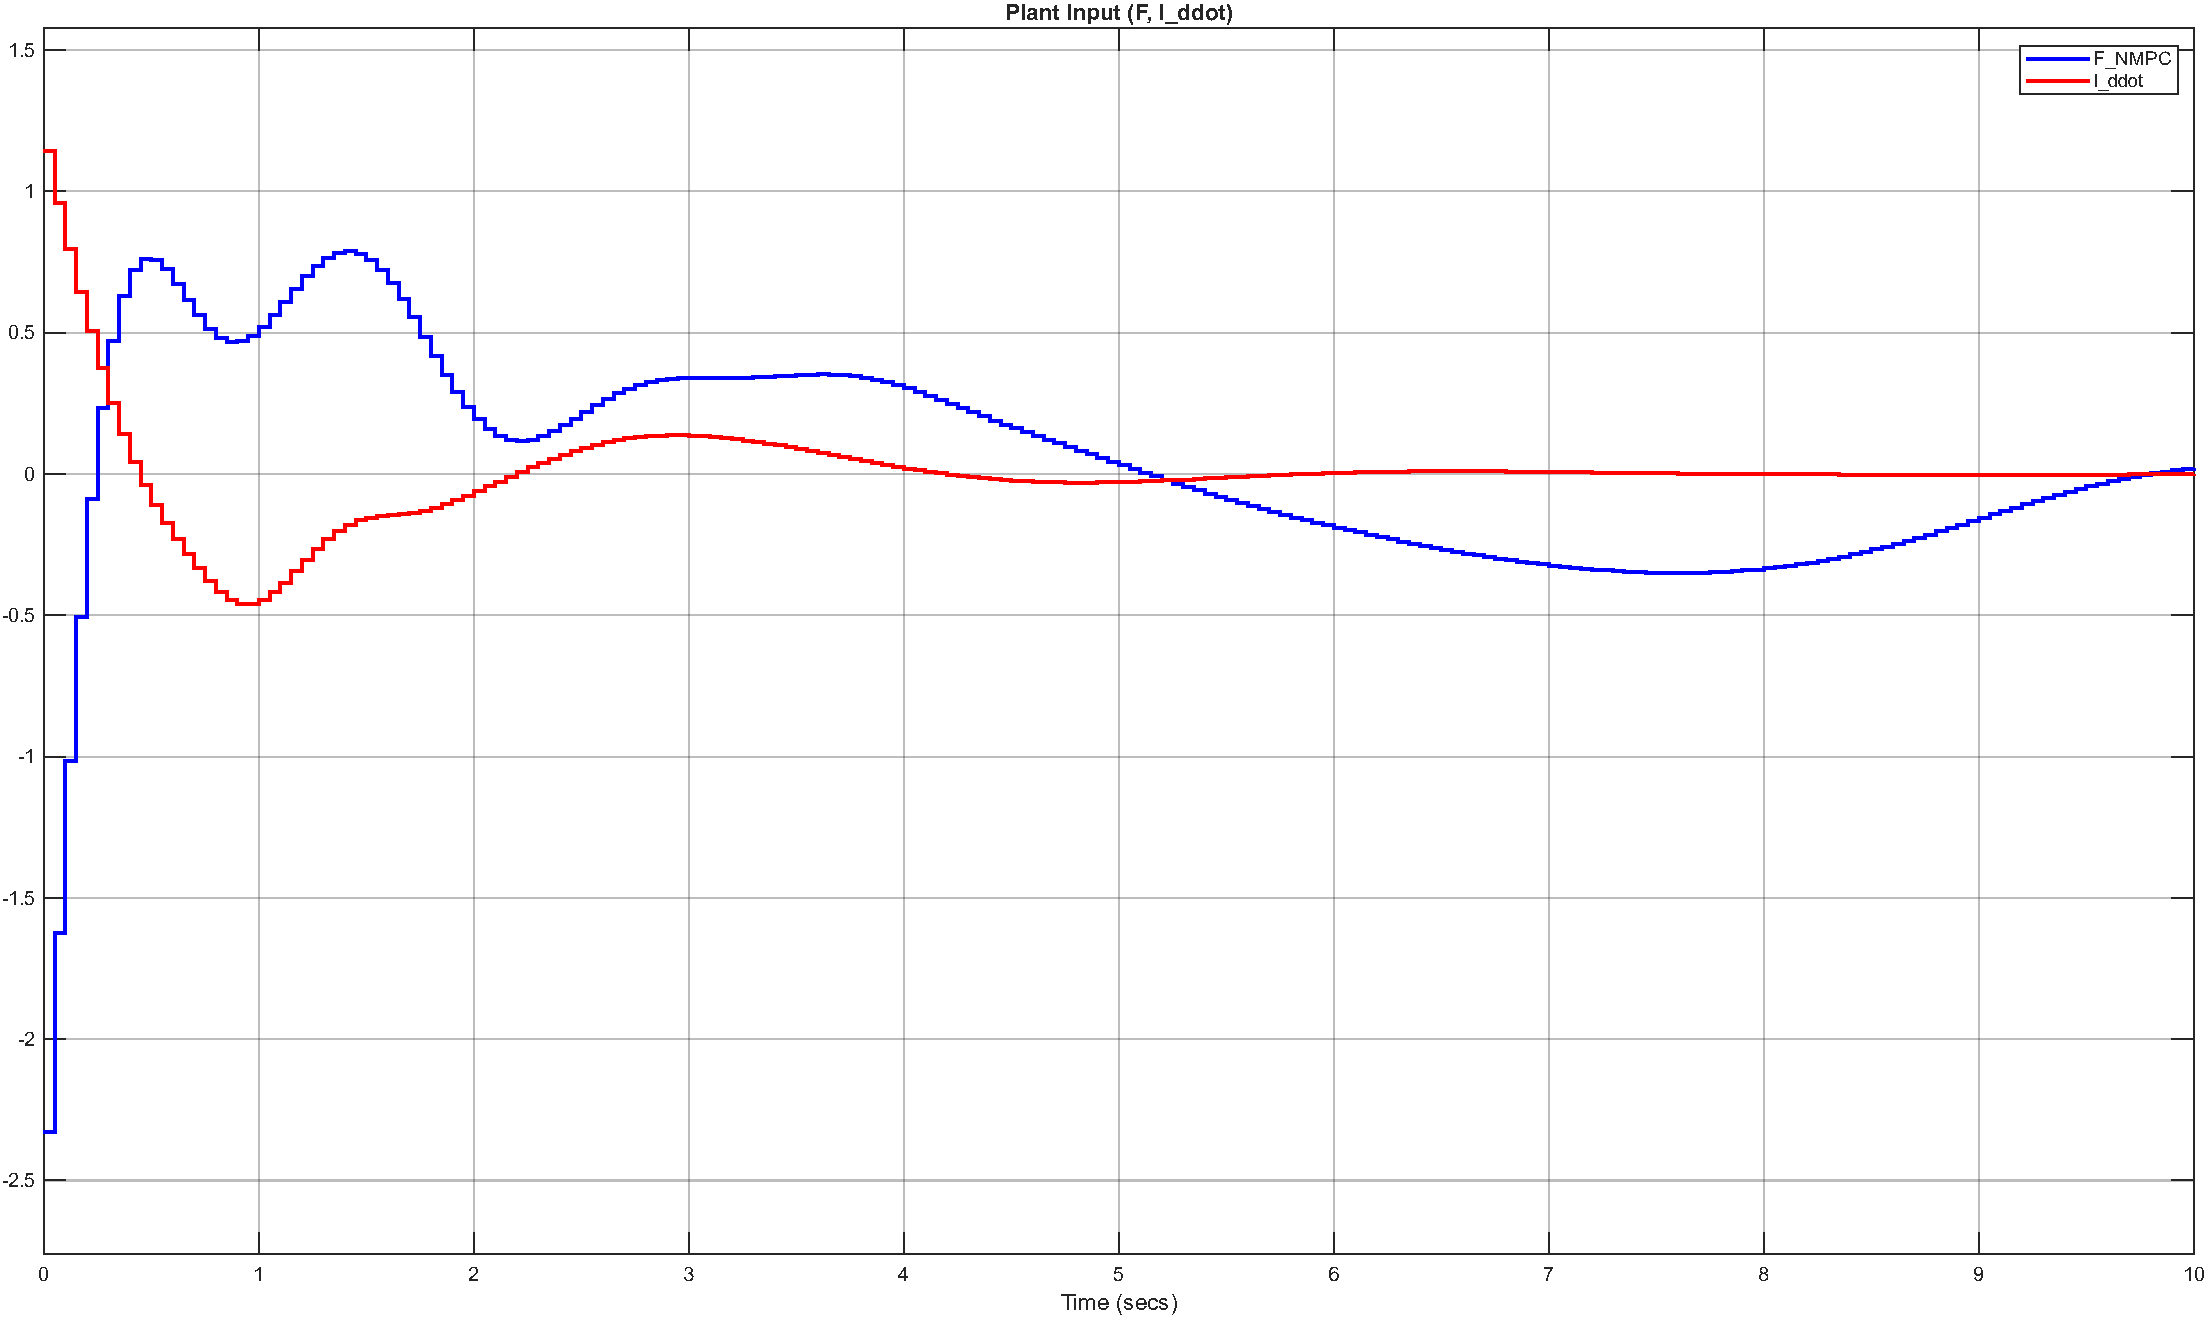
\includegraphics[width=0.85\textwidth]{images/4_NMPC_Trajectory/MPC_TRAJ_f_l_ddot_5.pdf}
    \caption{مدیریت ایمن عملگرها در شبیه‌سازی جابجایی بلندبرد ۵ متری}
    \label{fig:nmpc_traj_5_inputs}
\end{figure}